\documentclass{article}
\usepackage{amsmath}
\usepackage{ctex}
\usepackage{graphicx}
\usepackage[utf8]{inputenc}
\usepackage{geometry}
\usepackage{pdfpages}
\usepackage{hyperref}
\hypersetup{hypertex=true,
            colorlinks=true,
            linkcolor=blue,
            anchorcolor=blue,
            citecolor=blue}
%以下是为了展示python代码引入的包
\usepackage{listings}
\usepackage{color}
\usepackage{float} %指定图片位置
\usepackage{subfigure}%并排子图 共享标题 有子标题
\usepackage{caption}
\usepackage{amssymb}

\definecolor{dkgreen}{rgb}{0,0.6,0}
\definecolor{gray}{rgb}{0.5,0.5,0.5}
\definecolor{mauve}{rgb}{0.58,0,0.82}

\lstset{frame=tb,
  language=Python,
  aboveskip=3mm,
  belowskip=3mm,
  showstringspaces=false,
  columns=flexible,
  basicstyle={\small\ttfamily},
  numbers=none,
  numberstyle=\tiny\color{gray},
  keywordstyle=\color{blue},
  commentstyle=\color{dkgreen},
  stringstyle=\color{mauve},
  breaklines=true,
  breakatwhitespace=true,
  tabsize=3
}
%以上是为了展示python代码引入的包

\geometry{a4paper,scale=0.79}
\date{}
\title{双酚BPTK报告文档}
\author{许敬然}
\begin{document}
\maketitle
\section*{当前可用于展开的原始资料与基本情况说明}

当前我共从章学长处拿到一份微分方程组形式的PBTK模型,两份模型求解的R语言代码,包含各类参数。其中有两版不同的模型。

较早期的一版模型出于章学长的论文,形式是一份粘贴在word文档的R代码,里面用R语言中ode()求解器求解了63个变量关于时间的曲线。其中只有26个变量是实际所需求解的对象,它们存在有实际意义的关于时间的导数,剩余的变量只作为计算中间量。这些中间量可能并不存在关于时间的导数,
甚至有些变量并无实际意义,只是为了表示更方便,作为实际变量的导数表达式中的一部分出现。但是为了保证在求解器中的计算顺序准确,这些中间变量以某个虚构函数关于时间的导数信息的身份出现在求解器里,同其他导数信息共同被计算、求解。
例如涂抹时期内的用药剂量dose,实际上它在涂抹时期为一个正的常数,涂抹期过去后始终为0,但在代码中,它作为中间变量以“Rdose”的名字出现在了求解器的导数信息部分中。

此论文除了共享了部分模型求解代码,还共享了受试志愿者的部分生理参数
与尿液中非结合型双酚S的浓度与双酚S和双酚S-g的总浓度。代码里提供的参数与方程都来源于BPS(双酚S)(大部分方程与BPA(双酚A)在人体内的情况相同)。
其对应的实验情况是在四天内每一天同一时间令受试志愿者的手指与TP(Thermal-Paper热敏纸)持续接触,1分钟(涂抹时长)后停止触摸,此时手指上
有残留的BPs(双酚类物质)。130分钟(暴露时长)后用特殊试剂彻底清洗受试手指,此时表皮储仓内的BPs认为已清零,对应代码中的变量AWELL在13/6(h)处及后续的值与导数值置为零。与此同时,在受试期内,每260分钟取得一次受试者的尿液
并得到其中非结合型双酚S的浓度与双酚S和双酚S-g的总浓度。

后面一版模型都是关于BPA(双酚A)的,形式为一个有28个微分方程的方程组,其中除了第23、24个方程是非线性外,其他都是线性的。模型中的部分生理生化参数并未延续上述论文中的数值,而是有所更改。与之联系的代码是陈老师和章学长共同讨论过的带指数exp格式的模型求解代码,由于
讨论搁置,该求解代码并不是最终完善版本。
该版本的模型对应的实验情况有两种,其中第一种与上述论文中的实验方法相同,都是令手指与TP接触,涂抹时间都是1分钟,暴露时长(从开始涂抹到清洗)改为60分钟。
第二种是PCP(Personal-Care-Product个人护理产品)手臂暴露,四天内每12小时令受试者手臂涂抹PCP一分钟,留置6小时后彻底清洗,表皮储仓内的BPs清零。由于受试部位不同,两种暴露实验所使用的
皮肤参数有多出不同。该研究没有包含真实受试者数据。

\section*{早期模型求解代码(BPS)的Python复现与结果验证}

早期代码使用的部分人体生理参数来源于真实的受试者数据(受试者编号A),皮肤参数的设定基于手指皮肤。将链接文件的读取和参数平移至Python中,将变量与导数信息输入至scipy.integrate包中的的odeint求解器内求解。
求解的时间序列为arange(0, 75, 0.005),从零到第75小时,每18秒为一个节点,共15000个节点。所有变量的初值都为0。
之后将R代码中计算模型得到的结果(15001*64格的csv文件,其中第一列为时间序列)读取至Python中与Python的计算结果对比。

在求解时,最初我把源代码中63个变量精简为了26个变量,并未把原模型的中间变量放入求解器的导数信息中,而是把中间变量的计算公式放在了导数信息之外。这样的操作会导致在时间序列走完一步,26个变量都更新完数值后,中间变量才被计算,
设有变量的计算公式为$u_t=f(u_{t-1},\theta_t)$,其中$\theta$是中间变量,计算公式设为$\theta_t=g(v_t)$,如果按照我刚刚的这种操作方式,中间变量在求解迭代一轮结束后单独计算,$u_t$的计算
需要使用到$\theta_t$的信息,但是能拿到最新的$\theta$只能是$\theta_{t-1}$,故误差出现了。
该代码与源代码血浆内BPS浓度随时间变化曲线的对比结果如图\ref{fig:main}。

\begin{figure}
  \centering
  \subfigure[两种结果的绝对误差曲线]{
      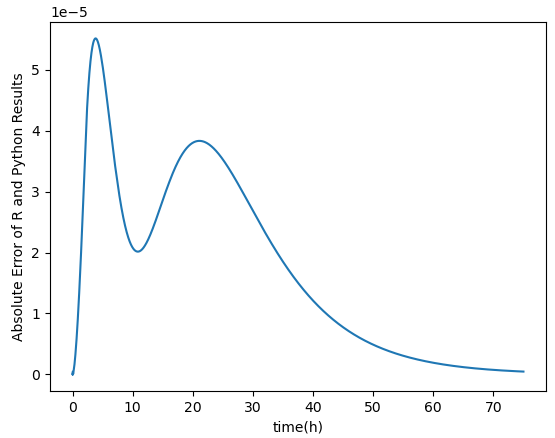
\includegraphics[width=0.45\textwidth]{pic2_1.png}
      \label{fig:subfig11}
  }
  \subfigure[两种结果的相对误差曲线]{
      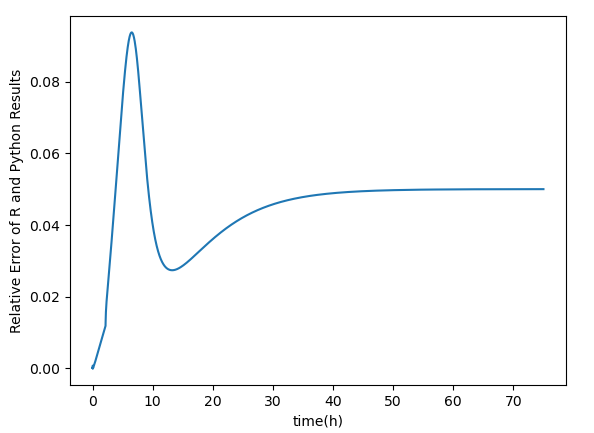
\includegraphics[width=0.45\textwidth]{pic2_2.png}
      \label{fig:subfig21}
  }
  \caption{源代码与复现代码A计算的血药浓度对比}
  \label{fig:main}
\end{figure}

可以发现绝对误差曲线的趋势与原曲线类似且较为光滑,相对误差的最大值超过了8\%。察觉到错误后,我又将中间变量作为导数信息放在了求解器中,得到的对比结果如图\ref{fig:main2}。
\begin{figure}
  \centering
  \subfigure[两种结果的绝对误差曲线]{
      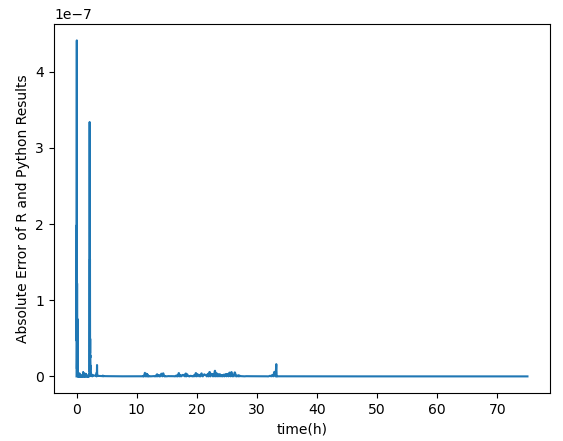
\includegraphics[width=0.45\textwidth]{pic1_1.png}
      \label{fig:subfig12}
  }
  \subfigure[两种结果的相对误差曲线]{
      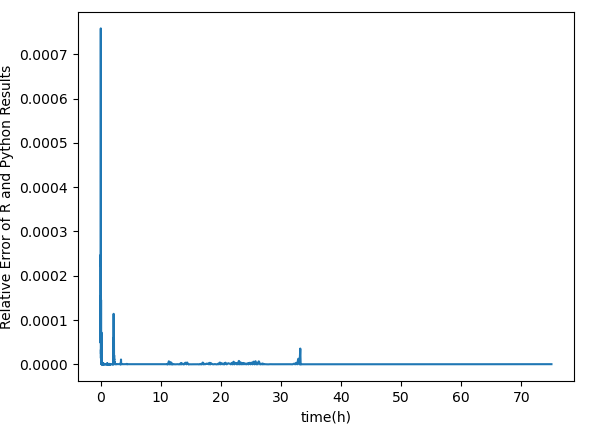
\includegraphics[width=0.45\textwidth]{pic1_2.png}
      \label{fig:subfig22}
  }
  \caption{源代码与复现代码B计算的血药浓度对比}
  \label{fig:main2}
\end{figure}
可以看到这份代码与源代码得到的结果几乎是相同的。

\section*{28方程求解模型(BPA)的Python复现与问题}

我拿到的基于28方程模型的R代码并没有使用求解器(带指数的迭代格式),在复现时,我使用了求解器求解28方程,得到的结果与R代码大相径庭。我又试着用BPS的模型代码求解(上一段有63个变量的求解器),部分参数改成BPA的参数(BPA
和BPS在人体内的代谢高度相似,只有部分参数不同),得到的结果也与28方程模型相差极大,三种方法得到的结果对比如图\ref{fig3}。
\begin{figure}[H]
  \centering
  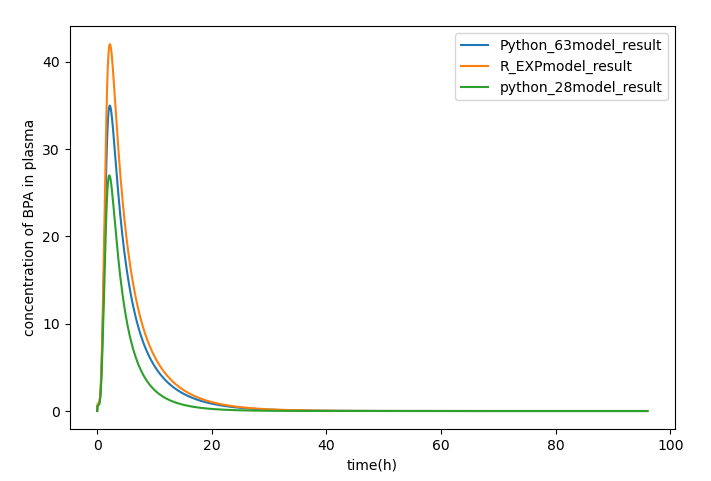
\includegraphics[scale=0.5]{pic3.png}
  \caption{三种代码的结果对比}
  \label{fig3}
\end{figure}

用求解器直接求解28方程组的结果与R代码中的指数格式不同是可以理解的。因为第23与24个方程并非线性方程,而在R代码中对这一点做了求解上的近似:在用积分因子法导出这两个方程的计算格式时,
将非线性部分视为了常数部分,只使用了线性部分,像其他线性方程一样导出了相同的带指数的格式。这样的近似带来了偏差是合理的。

但28方程模型实际上是对63变量求解法的整理,去除了绝大部分中间变量,将所求变量精简到了28个。但用求解器直接求解这28个方程是会出现错误的,例如第24个变量Aliver,代表了肝脏中化学品含量,
按理说应该始终是非负值,但是求解得到的结果一直是非正的。我试着用R中的求解器deSolve包内的ode()求解28方程组,得到的结果(血浆药浓度、肝脏药浓度)都与Python内求解器得到的结果高度相似,结果如图\ref{fig:main4}。

\begin{figure}
  \centering
  \subfigure[两种血药浓度的相对误差]{
      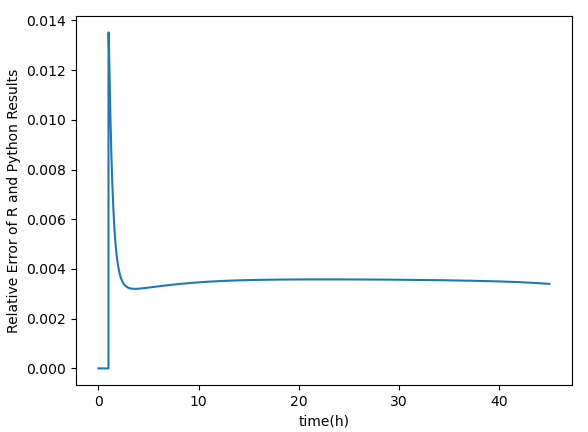
\includegraphics[width=0.45\textwidth]{pic4_1.png}
      \label{fig:subfig41}
  }
  \subfigure[两种肝脏药浓度的相对误差]{
      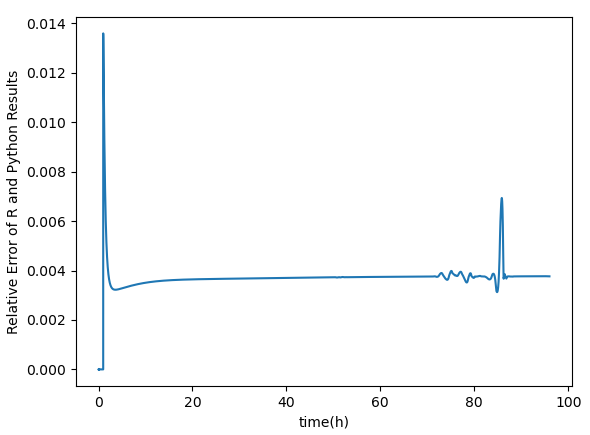
\includegraphics[width=0.45\textwidth]{pic4_2.png}
      \label{fig:subfig42}
  }
  \caption{R与Python求解28方程计算结果对比}
  \label{fig:main4}
\end{figure}

可以看到在求解28方程组时,R中求解器也出现了得到异常负值的情况。且根据两种求解器得到的血药浓度的高度一致可以断定,负值错误的发生与求解器本身没有关系,而是28方程组本身出现了问题。
用63变量模型求解得到的肝脏药浓度是正值,且看起来和28方程模型求得的肝脏药浓度的绝对值很接近,事实上,这二者间的相对误差很高。部分结果如图\ref{fig:main5}。


\begin{figure}
  \centering
  \subfigure[几种方法得到的肝脏药浓度曲线]{
      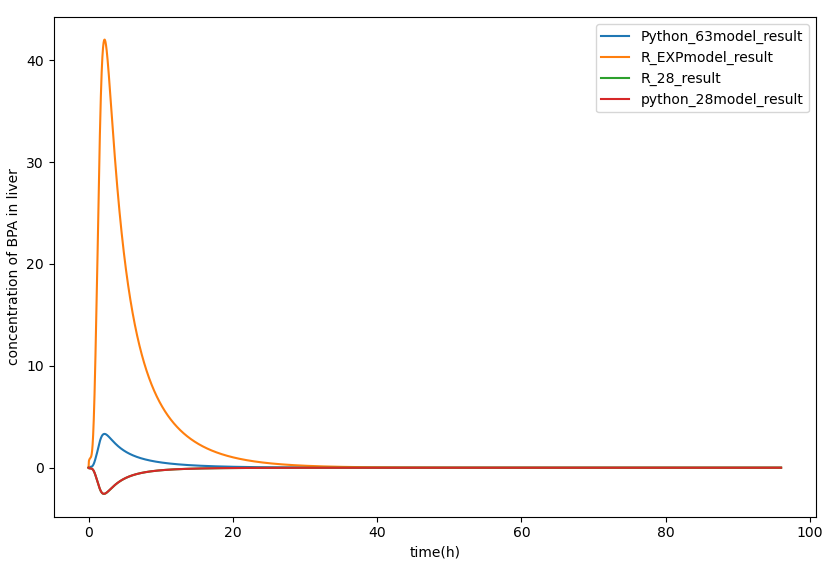
\includegraphics[width=0.45\textwidth]{pic5_1.png}
      \label{fig:subfig51}
  }
  \subfigure[28法与63法得到的肝脏药浓度的绝对值的绝对误差]{
      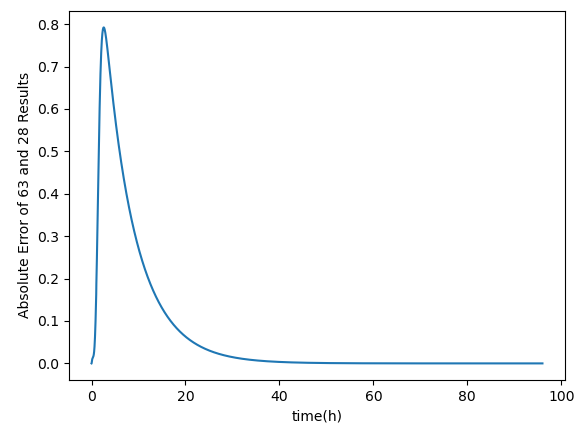
\includegraphics[width=0.45\textwidth]{pic5_2.png}
      \label{fig:subfig52}
  }
  \subfigure[28法与63法得到的肝脏药浓度的绝对值的相对误差]{
      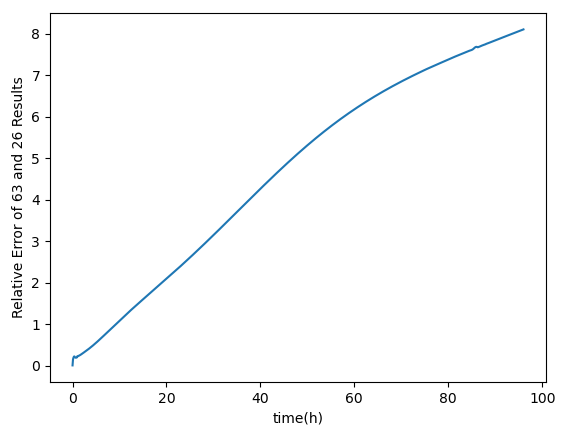
\includegraphics[width=0.45\textwidth]{pic5_3.png}
      \label{fig:subfig53}
  }
  \caption{不同结果得到的肝脏药浓度结果对比}
  \label{fig:main5}
\end{figure}

28方程组需要进一步讨论与解析,目前的版本得到的血药浓度的变化趋势是正确的,但由于缺少一个正确的对照,并不清楚实际数值是否在可接受范围之内。同时,该版本得到的
肝脏药浓度曲线是错误的,而基于28方程组得到的带指数的格式计算出的肝脏药浓度是正的。是否由于第23,24个方程的非线性部分造成两个结果的不同需要进一步探究。

\section*{三参数优化的Python复现(基于BPS模型)}

在后续与章学长的交流中,我拿到了一份基于BPS模型的参数优化代码。本文档的第一部分提到过,在BPS的人体BPTK模型研究中对受试者每隔4.3333小时采一次尿,以测量尿液中的未结合BPS含量和BPS\&BPS-g的总含量。
他们的优化参数的做法即是,使用R中的optim()函数在三参数的情况下最小化损失函数(三个参数:DSC<角质层中的有效扩散系数>、PFO<毛囊的渗透系数>、u1<由脱屑而向皮肤表面转移的速度>)。
其中损失函数是真实测量数据的时间序列和模型计算出的与之对应时间节点的尿药浓度之间的SSE(误差平方和)。有效受试者共有四位,损失函数中的SSE是四名受试者对应SSE的总和。

我首先准备复现这个优化算法。最开始,我选择了使用scipy.optimize包中的minimize()函数来最小化损失函数,尝试了函数中的许多methods,但几乎不奏效。
接下来换了另一个适用于调整超参数的优化函数hyperopt.fmin(),得到了更显著的优化结果,但SSE依旧很大(原始R代码优化后参数对应的SSE也很大),得到过最好的优化结果对应的SSE$\approx$21。

完成原始优化参数代码复现的第二天,在论文讨论班里,陈老师说参数优化的最终目的是,当输入为离散的血药浓度数据时,能快速得到对应的三个目标参数的大概取值。
在清楚这个目标后,我放弃了从这份复现代码继续考虑下去。


\section*{基于LSTM神经网络模型的参数反演(BPS模型)}

在清楚参数优化的当前目的后,根据陈老师所建议的神经网络模型路径,我尝试搭建了一个神经网络,数据集内的输入数据为通过BPS的BPTK模型计算得到的血药浓度曲线中的离散点组,标签为对应的三个待优化参数.
训练结束后保存最优模型,将已有数据集之外的数据代入网络,再用得到的三参数通过BPTK模型正向计算血药浓度曲线,最终比较二者的误差。得到了较为合理的结果。以下是详细介绍。

\subsection*{数据集的搭建}
我想得到10000组数据。首先,我需要得到10000组不同的三参数组合,对每种参数在其合理的取值范围内离散地取$N_i(i=1,2,3)$个样,令$N_1\times N_2\times N_3=10000$。
根据已有的参考资料中的实际取值与上一个部分中我复现的参数优化代码得到的参数取值,我将三个参数的取值范围界定为:$DSC_0\in (10,40),PFO_0\in (0,15),u_1^0\in (0,15),(其中DSC_0\triangleq DSC
\times 10^{-9},PFO_0 \triangleq PFO\times 10^{-5},u_1^0\triangleq u_1\times 10^{-5})$。又考虑到三个参数在这个取值范围内仍有一个更合理的取值范围,设置参数在更合理的区间内频次更高地等距取点,
例如我为$DSC_0$设置了三个取样区间,在$(15,20)$中(严格地)每隔0.5取一次点,在$(10,15)\cup (20,30)$中每隔1.2取一次点,在$(30,40)$中每隔4取一次点,在后两个区间的取点间隔不一定严格遵守,而是根据实际情况
进行了更合适的调整。$DSC_0$共取样25个,$PFO_0$与$u_1^0$各取样20个,取三个一维数组的笛卡尔积后便可以得到10000组不同的三参数组合。这10000个含有三个浮点数的一维数组,合起来后是一个10000*3的二维数组,即是数据集中的标签数据label。


接下来是输入数据的搭建。对range(0,75,0.005)共15000个时间节点进行取样以模拟定时抽血化验。希望对时间序列的取样可以含有尽可能多的信息,同时考虑到计算量需要尽可能精简取样点的数量。如图\ref{fig6},
曲线的曲率在前20个小时有较大的变化,而20时后曲率的变化率放缓,曲率也减小。可粗略认为前二十小时内的曲线相较于二十小时后承载了更密集的信息量,这和现实世界中的常识也是吻合的,在给药后人们总是更密切频率更高地
监测离给药节点更近时的实验体数据。因此,设定从0.5时至20时结束,每0.5小时取一次样;从20.5时至74.5时结束,每2小时取一次样。总共得到68个时间取样点。
将10000个不同的三参数数组分别代入至BPS的BPTK模型中,使用1号受试者的部分生理参数,计算得到10000组血药浓度曲线。取每一个血药浓度曲线在上述68个时间节点处对应的浓度值,得到10000个含有63个浮点数的一维数组,合起来即是一个10000
*68的二维数组,即是数据集中的输入数据。至此即完成了数据集的搭建。
\begin{figure}[H]
  \centering
  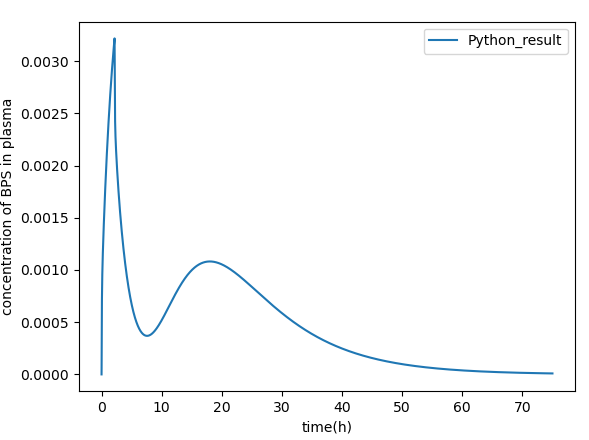
\includegraphics[scale=0.5]{pic6.png}
  \caption{计算63变量模型得到的血药浓度曲线}
  \label{fig6}
\end{figure}



\subsection*{神经网络模型的搭建}

一条输入数据是68个有顺序的时间采样点对应的血药浓度值,是一个时间序列。在这样一个数组中,某个时间点对应的数值$C^{plasma}_{t_{n}} = f(\;\cdot\; ,C^{plasma}_{t_{n-1}},\cdots,C^{plasma}_{t_{0}})$。
循环神经网络(Recurrent Neural Network)能够捕捉到时间序列的自相关信息,而作为RNN架构的升级版, 长短期记忆循环神经网络LSTM(Long Short Term Memory)能够在理解简单的时间滞后信息的同时捕捉到更大更广的随时间
变化的趋势。因此我选择了两层的LSTM网络作为隐藏层的前两层。其中第二层设置了一个dropout率为0.2的dropout。LSTM层的输入信息为一个$batchsize*68*1$三维张量,其中第三维度的“1”代表这个时间序列只有一个特征维度,即是血药浓度。输出结果之一
是一个$batchsize*68*128$的三维张量(剩余的输出结果后续不需要)。取三维张量第二维中的最后一个元素所对应的二维张量,作为下一层的输入信息。
接下来是两层连续的全连接层,第一层的输入信息为一个$batchsize*128$的二维张量,输出信息(第二层全连接的输入信息)为一个$batchsize*64$的二维张量。
最终整个网络的输出信息为一个$batchsize*3$的二维张量,代表了$batchsize$组由网络计算得到的三参数组合。

\subsection*{训练验证与测试}

首先,对输入数据10000*68的二维数组进行标准化,对于每一列$X^{norm}_i=\frac{X_i-\mu(X_i)}{\sigma(X_i) } $。
接下来,在10000组输入数据与对应标签中,不放回地抽取其中的8000组数据作为训练集,继续不放回地抽1000组数据作为验证集,剩下的1000组数据作为测试集。

训练的目标loss函数是输出数组与标签数组之间的均方误差MSE(Mean Squared Error)。
优化器使用的是torch.optim中的Adam()。Adam优化算法中的下降步长需要使用当前梯度信息的一阶矩估计(梯度信息的指数平滑)与二阶矩估计(梯度信息的逐项平方的指数平滑)。矩估计在经过
修正后(时间步较小时的矩估计将会被放大),代入至更新步公式$\Delta \theta   = -\epsilon \frac{\hat{s}}{\sqrt{\hat{r}} +\delta } $,其中$\hat{s}$为修正后的一阶矩估计,$\hat{t}$
为修正后的二阶矩估计,$\delta$为用于数值稳定的小常数。Adam算法有以下优点:梯度下降步长随梯度信息而变化,并且这种变化能捕捉到梯度信息的变化趋势;
对矩估计的修正有着模拟退火算法的效果,在迭代早期更容易跳出局部最优;使用一阶动量与二阶动量,在相同的梯度方向能积累速度,等等。

设置训练epoch为200,使用小批量训练的方式,$batchsize = 32$。在训练迭代中设置early stopping机制,当验证集上的loss低于某个值时开启early stopping模式,当距离上一次最优loss已经$n$个迭代步数
时停止训练,并储存最优loss对应的模型。最后将测试集代入最优模型来查看泛化效果。



\subsection*{结果展示与效果对比}
若模型在测试集上效果较好,则在另一个测试文件中用未出现在10000组数据集中的三参数正向生成一条曲线,并按照已有规则在曲线
上取得68个取样点,代入至已储存模型中计算反演的三参数。利用反演出的三参数正向生成一条曲线,将得到了两条曲线共同绘出,并绘制它们之间的绝对误差、相对误差曲线,以此来对比结果。



\end{document}